%Lab4
\section{Circuit description}
\label{sec:analysis}

\begin{figure}[h] \centering
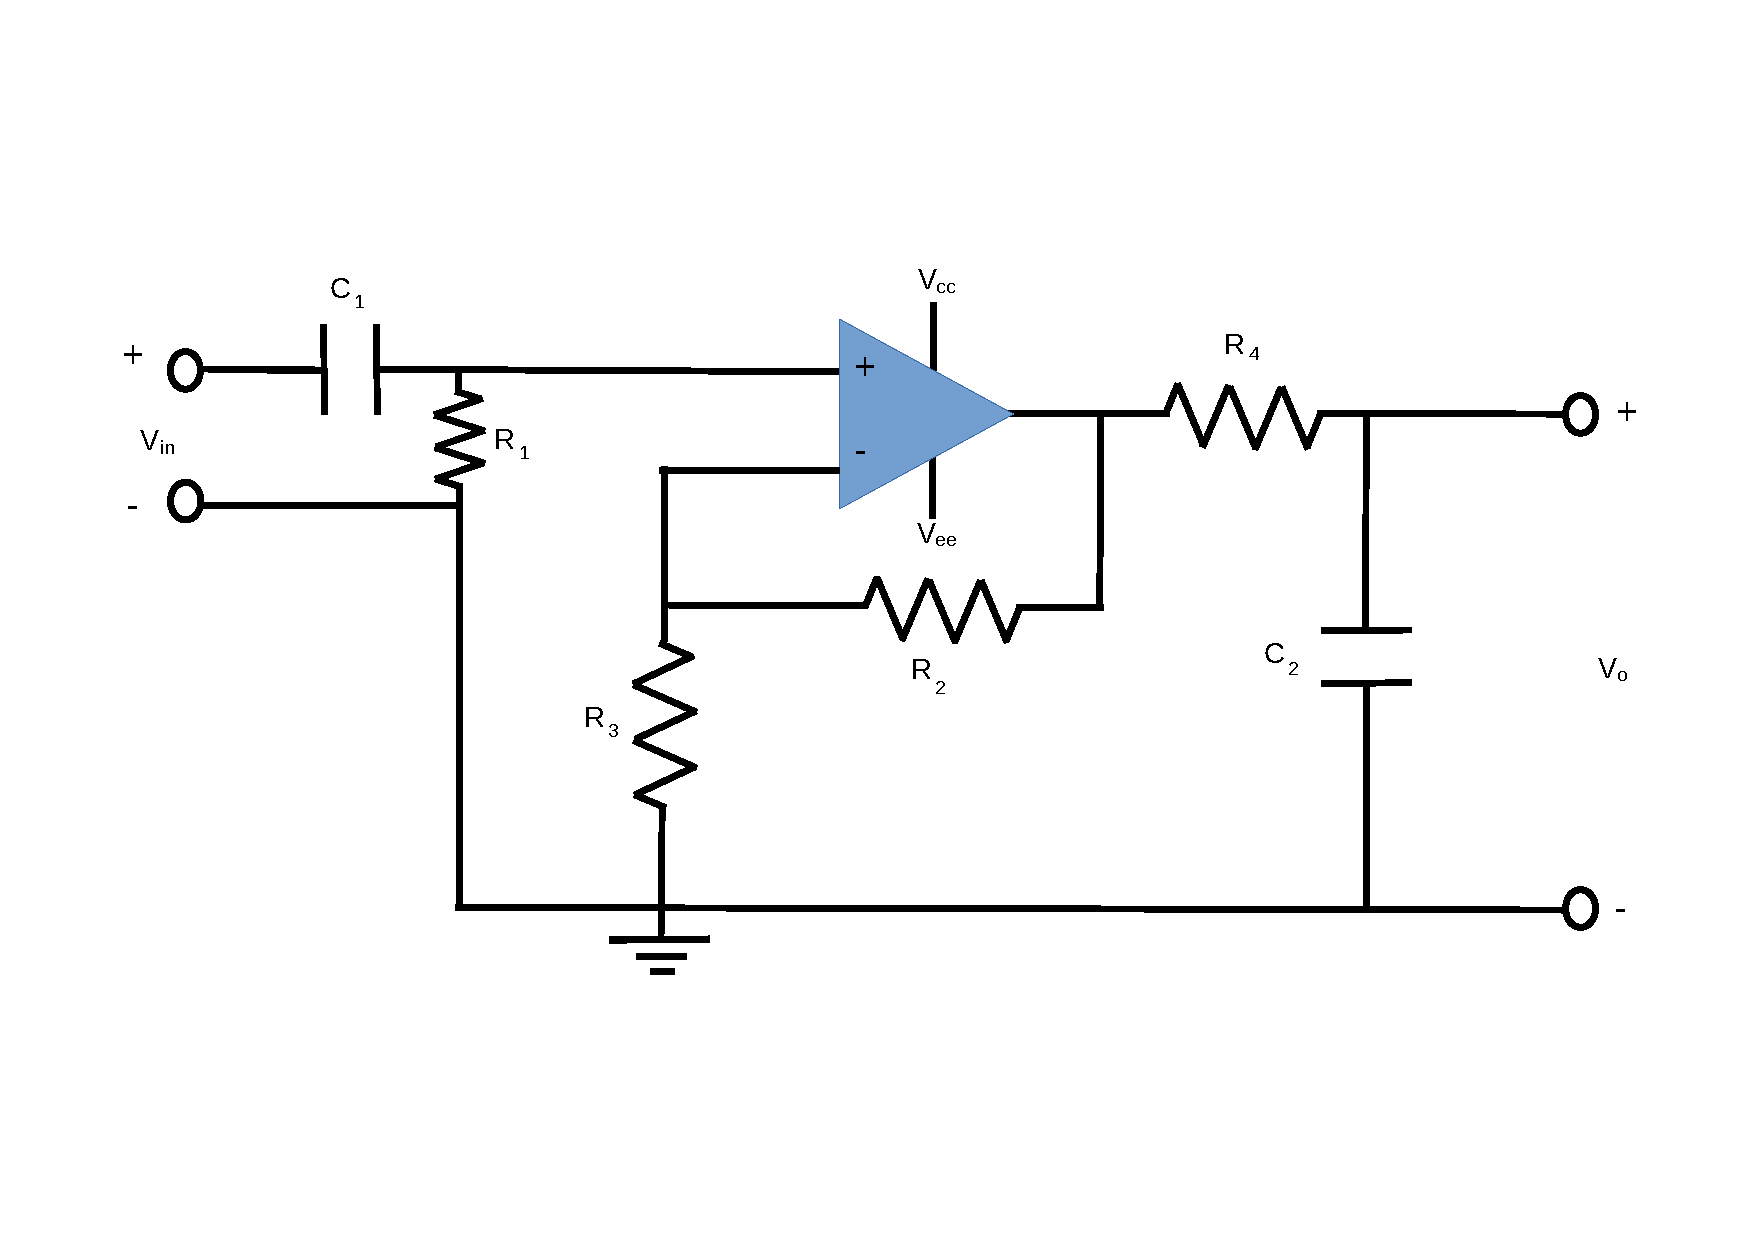
\includegraphics[width=0.9\linewidth]{../figlib/t5.pdf}
\caption{Circuit to be analysed in this report.}
\label{fig:lab4}
\end{figure}


\par In the current section, we will describe the circuit shown in Figure \ref{fig:lab4}. 
So in this circuit you can see our final configuration to build a bandpass filter. It is composed by 1 input voltage source, 1 OP-AMP uA741, 4 resistors $R_{1}$, $R_{2}$,
$R_{3}$ and $R_{4}$ and 2 capacitors $C_{1}$ and $C_{2}$.
\par In the table \ref{tab:circuit_values} it can be seen all the components and their respective values.


\begin{table}[h]
  \centering
  \begin{tabular}{|l|r|}
    \hline    
    {\bf Name} & {\bf Value [{$\Omega$} or V or F]} \\ \hline
    \input{../mat/Values.tex}
  \end{tabular}
  \caption{Values of the various components and parameters.}
  \label{tab:circuit_values}
\end{table}

To obtain a value of $R_{2}$, which needs a subcircuit, we used a series of one 100K$\Omega$ resistor with a parallel of two 100k$\Omega$ resistors. 

\begin{equation}
R_2 = 100+\frac{1}{\frac{1}{100}+\frac{1}{100}} k\Omega
\end{equation}

To obtain a value of $C_{2}$, which needs a subcircuit, we used a series of two 220nF capacitors.

\begin{equation}
C_2 = \frac{1}{\frac{1}{220}+\frac{1}{220}} nF
\end{equation}

\newpage
\section{Circuit Analysis}
\label{sec:circuit}
\subsection{Theoretical analysis}
\label{sub:t1}

\par In this subsection, the circuit shown above is analysed theoretically using octave to make the calculations.

To start with, we only had to analyse the gain and the impedances (input impedance and output impedance). In order to make the gain easier to understand we  started by both
impedances. Analysing the circuit we compute the input impedance:

\begin {equation}
ZI = R_1 + \frac{1}{j \cdot w \cdot C_1}
\label{eq:1}
\end {equation}

Then to compute the output impedance: 

\begin {equation}
ZO = R_2||\frac{1}{j \cdot w  \cdot C_2}||R_4
\label{eq:2}
\end {equation}

\par In the table \ref{tab:1} we present the results for input and output impedances (assuming central frequency 1000 Hz) using the previous equations and octave.

\begin{table}[h]
  \centering
  \begin{tabular}{|l|r|}
    \hline    
    {\bf Name} & {\bf Value [{$\Omega$}]} \\ \hline
    \input{../mat/Impedances.tex}
  \end{tabular}
  \caption{Impedances at 1000 Hz.}
  \label{tab:1}
\end{table}

\par After computing impedances, we must compute the gain. The gain is given by the following expressions:

\begin {equation}
Gain = A_V\cdot A_H \cdot A_L
\label{eq:31}
\end {equation}

\begin {equation}
A_V = 1+\frac{R_2}{R_3}
\label{eq:32}
\end {equation}

\begin {equation}
A_H = \frac{j*w*C_1*R_1}{1+j*w*C_1*R_1}
\label{eq:33}
\end {equation}

\begin {equation}
A_L = \frac{1}{1+j*w*C_2*R_4}
\label{eq:34}
\end {equation}

Where $A_{V}$ is the gain related to the OP-AMP, $A_{H}$ is the gain related to the first stage where we have an highpass filter and $A_{L}$ is the gain related to the
final stage where we have a lowpass filter.

\par And using the previous equations we obtained the gain presented in the table \ref{tab:2} (assuming central frequency 1000 Hz).

\begin{table}[h]
  \centering
  \begin{tabular}{|l|r|}
    \hline    
    {\bf Name} & {\bf Value [dB]} \\ \hline
    \input{../mat/Gain.tex}
  \end{tabular}
  \caption{Gain at 1000 Hz.}
  \label{tab:2}
\end{table}

\par To better understand the frequency response of gain, we plot the following graph \ref{fig:11}, where we can see that low and high frequencies have a low gain and 
frequencies near to 1000 Hz have the maximum gain. This happens because in the first stage we have an highpass filter that blocks low frequencies and in the final
stage we have a lowpass filter that blocks high frequencies. To ensure an high gain, we must focus obtaining an high $A_{V}$, because near the central frequency both $A_{H}$
and $A_{L}$ will be as close as possible to 1. 
We can see aswell in graph \ref{fig:12} the plot for the theoretical phase of the output voltage which is similar to a normal bandpass filter. 

\begin{figure}[h!]
           \centering
           \subfigure[]{\includegraphics[width=0.45\textwidth]{gain1.eps}\label{fig:11}} 
            \subfigure[]{\includegraphics[width=0.45\textwidth]{phase1.eps}\label{fig:12}}
           \caption{(a) Gain in frequency response (b) Phase in frequency response}
           
\end{figure}

%\newpage

\subsection{Simulation analysis}
\label{sub:s1}

\par In this subsection, the circuit shown above is simulated with ngspice.

As in the previous subsection we have to analyse the gain and the impedances, as well as the central frequency.
We start by the impedances. \par To simulate in ngspice the input impedance, we must measure the voltage drop between ground and the input voltage source, and then 
we divide it by the current that goes through the input voltage source. To simulate the output voltage, we did other script where we turned off the input voltage source 
and added a voltage source in between $v_{o}$ and ground.  
\par The results obtained are presented in the tables \ref{tab:3} and \ref{tab:4} and impedances are calculated to 1000 Hz, which is the desired central fequency.

\begin{table}[h]
  \centering
  \begin{tabular}{|l|r|}
    \hline    
    {\bf Name} & {\bf Value [{$\Omega$}]} \\ \hline
    \input{../mat/tablezi_tab.tex}
  \end{tabular}
  \caption{Input Impedance at 1000 Hz.}
  \label{tab:3}
\end{table}

\begin{table}[h]
  \centering
  \begin{tabular}{|l|r|}
    \hline    
    {\bf Name} & {\bf Value [{$\Omega$}]} \\ \hline
    \input{../mat/tablezout_tab.tex}
  \end{tabular}
  \caption{Output Impedance at 1000 Hz.}
  \label{tab:4}
\end{table}

\par After simulating impedances, we plotted the gain in frequency response as we can see in figure \ref{fig:31} and the plot is similar to the theoretical analysis, being the 
reason the same as before, - it can be seen in the subsection \ref{sub:t1} - the filters are blocking low and high frequencies and the high quocient of $\frac{R_{2}}{R_{3}}$ 
allows to have a band with high gain - where central frequency is close to 1000 Hz. 
The gain plot is followed by the phase plot \ref{fig:32} of the output voltage, which will be further explored while comparing the theoretical and simulation results.

\begin{figure}[h!]
           \centering
           \subfigure[]{\includegraphics[width=0.40\textwidth]{gaint.pdf}\label{fig:31}} 
            \subfigure[]{\includegraphics[width=0.40\textwidth]{phase.pdf}\label{fig:32}} 
           \caption{(a) Gain in frequency response (b) Phase in frequency response}

\end{figure}

\vspace {5cm}

\par Nevertheless, we had to compute the central frequency in order to later calculate its deviation. To do this we measured the maximum value of the gain and calculated the frequencies where 
the gain would be 3 dB lower. Finally to obtain the central frequency we did a geometric average - $\sqrt{(low cut off frequency)\cdot(high cut off frequency)}$ - obtaining the following set of 
values - table \ref{tab:5}:

\vspace {1cm}

\begin{table}[h]
  \centering
  \begin{tabular}{|l|r|}
    \hline    
    {\bf Name} & {\bf Value [{$\Omega$}]} \\ \hline
    \input{../mat/tablefrequencies_tab.tex}
  \end{tabular}
  \caption{Central frequency.}
  \label{tab:5}
\end{table}




\subsection{Comparation of results} 
\label{sub:comp}

In this subsection we will compare the results of the two previous subsections \ref{sub:t1} and \ref{sub:s1}, more concretely we will compare the gain and the impedances.
\par Starting with the impedances, both impedances are similiar in theoretical and simulation analysis, because the OP-AMP is not perfect and ngspice uses a more complex
models to analyse it.
\par Then looking to the gain response, we can see that both of them are similar, but since ngspice uses more complex methods to obtain the gain,
we find some differences between them, being important the central frequency and the maximum gain value. 
\par To finish, as we already said, we are going to compare the phase plots of both analysis. In octave we find one root and two poles because of the presence of two capacitors, but 
in ngspice, we have one root and four poles. It is consequency of the OP-AMP, in octave we consider it as an ideal one, but in fact the OP-AMP has two capacitors that produce
two more poles and, since ngspice uses more complex models to components, it is capable of using this information to create more accurate analysis.


\newpage
\section{Discussion of results}
\label {sec:aspects}

In the past sections and subsections the circuit was analysed in order to calculate the final merit. Before this calculation we will explore some of the decisions made and the reason why. 
\par First of all, we must look at the merit formula, that is presented in the equation \ref{eq:merit}, so we know what improvements to make in order to increase it. 

\begin{equation}
M=\frac{1}{(cost) \cdot (gain deviation) \cdot (central frequency deviation)+10^{-6}}
\label{eq:merit}
\end{equation}

\par Looking at the formula \ref{eq:merit} we can say that in order to increase the merit we had to decrease all the parameters in denominator - the cost, the gain deviation and the central 
frequency deviation. So now it is important to study the impact of changing the components and their respective value of the parameters mentioned before. The use of 2 capacitors - $C_{1}$ and $C_{2}$ - was 
essencial to achieve a bandpass filter since on a first stage, where we couple the capacitor $C_{1}$ in series with $R_{1}$ shown in figure \ref{fig:21}, we produce an highpass filter, 
and on a second stage where we couple the $C_{2}$ in parallel with $R_{4}$ with shown in figure \ref{fig:21}, where we obtain a lowpass filter. Combining these two filters we obtain a bandpass filter as desired. 
Also it is worth mentioning that the capacitance values interfere in the 
obtained results mainly in the central frequency, this way the final values used were the ones that by experienced allowed us to maximize the quantities we needed to.
%By experience we saw that we could only achieve the 1000 Hz central frequency if we used an higher capacitance in capacitor $C_1$ than in capacitor $C_2$.

\begin{figure}[h!]
           \centering
           \subfigure[]{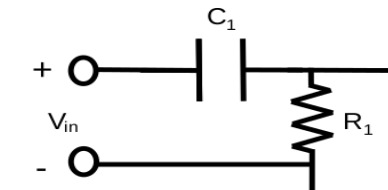
\includegraphics[width=0.40\textwidth]{../figlib/t5_2.jpeg}\label{fig:21}} 
            \subfigure[]{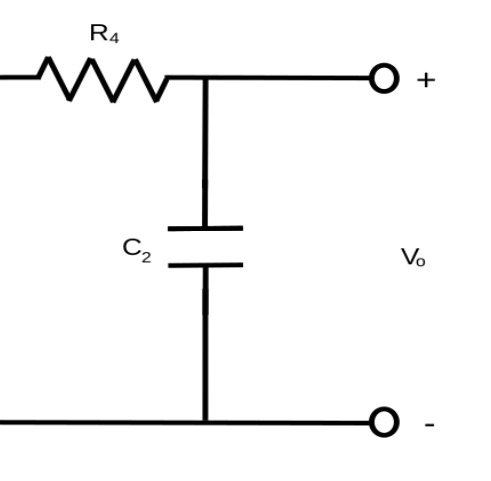
\includegraphics[width=0.35\textwidth]{../figlib/t5_1.jpeg}\label{fig:22}} 
           \caption{(a) Highpass filter section (b) Lowpass filter section}

\end{figure}


\par As for the resistances used their values were chosen keeping in mind the formulas that given the theoretical gain, being essential to have $R_{2}$ much higher than
${R_3}$. 
On the other hande, resistances ${R_1}$ and ${R_4}$ their values seek having the poles frequencies as close as possible to the central frequancy desired.
%\par As for the resistances used their values were chosen keeping in mind the formula that gives the theoretical gain - equation \ref{eq:31} - being essential that resistor $R_1$ was 100 
%times lower than the resitor $R_2$ to achieve 40 dB. We noticed aswell that their ratio wasn't the only thing to focus since if we increased them too much the central frequency would lower a lot, so
%the values used were achieved by experience in order to obtain both wanted gain and central frequency. 

The results we obtained to the various properties taken in account in the merit formula were the following:

\begin{table}[h]
  \centering
  \begin{tabular}{|l|r|}
    \hline    
    {\bf Name} & {\bf Value [dB or Hz or MU]} \\ \hline
    \input{../mat/tableall_tab.tex}
 	\end{tabular}
  	\caption{Circuit final results}
 	 \label{tab:merit1}
	\end{table} 

\par Looking to the results shown in table \ref{tab:merit1}, we can see that the gain was around the one we wanted aswell as the central frequency, which are close to 40 dB and 1000 Hz, while keeping the 
cost low. This results in a good merit considering all the tests done before. 
























